\documentclass[12pt,initial,twoside,maitrise]{dms}
\usepackage[utf8]{inputenc} %Obligatoires
\usepackage[T1]{fontenc}    %
\usepackage{minted}
\usepackage{array}
\usepackage{epigraph}
\usepackage{tikz}
\usepackage{tikz-qtree}
\usepackage[options ]{algorithm2e}

\def\sloppy{%
\tolerance 500%  %9999 dans LaTeX ordinaire, mauvaise idée.
\emergencystretch 3em%
\hfuzz .5pt
\vfuzz\hfuzz}
\sloppy   %appel de \sloppy pour le document
%%\fussy  %ou \fussy

%% Packages utiles.
\usepackage{graphicx,amssymb,subfigure,icomma}
%% icomma       permet d'écrire les nombres décimaux en
%%                  français (p.ex. 1,23 plutôt que 1.23)
%% subfigure    simplifie l'inclusion de figures côtes-à-côtes

%% Packages parfois utiles.
%%\usepackage{dsfont,mathrsfs,color,url,verbatim,booktabs}
%% dsfont       symboles mathématiques \mathds
%% mathrsfs     plus de symboles mathématiques \mathscr
%% color        pour utiliser des couleurs (comparer avec <xcolor>)
%% url          permet l'écriture d'url
%% verbatim     pour écrire du code ou du texte tel quel
%% booktabs     plus de macros pour faire les tableaux
%%                  (voir documentation du package)

%% pour que la largeur de la légende des figures soit = \textwidth
\usepackage[labelfont=bf, width=\linewidth]{caption}

%% les 3 lignes suivante servent à l'affichage de l'index
%% dans le visionneur de pdf. <hyperref> et <bookmark>
%% devraient être les dernier package a être chargé,
%% donc chargez vos packages avant.
\usepackage{hyperref}  % Ajoute les hyperlien
\hypersetup{colorlinks=true,allcolors=black}
\usepackage{hypcap}
\usepackage{bookmark}

\newtheorem{cor}{\corollaryname}[section]
\newtheorem{deff}[cor]{\definitionname}
\newtheorem{ex}[cor]{\examplename}
\newtheorem{lem}[cor]{\lemmaname}
\newtheorem{prop}[cor]{Proposition}
\newtheorem{rem}[cor]{\remarkname}
\newtheorem{theo}[cor]{\theoremname}

\numberwithin{equation}{section}
\numberwithin{table}{chapter}
\numberwithin{figure}{chapter}

\renewcommand{\baselinestretch}{1.5}

\begin{document}

\version{1}


\title{Programming tools for intelligent systems\\
\small{with a case study in autonomous robotics}}

\author{Breandan Considine}

\copyrightyear{Ann\'ee de la th\'ese}

\department{D\'epartement d'informatique et de recherche op\'erationnelle}

\president{Nom du pr\'esident du jury}

\directeur{Nom du directeur de recherche}

%%\codirecteur{Nom du co-directeur}         % s'il y a lieu

\membrejury{Nom du membre de jury}

%%\examinateur{Nom de l'examinateur externe}   %obligatoire pour la these

%% \membresjury{Deuxième membre du jury}  % s'il y a lieu

%%  \plusmembresjury{Troisième membre du jury}    % s'il y a lieu

%%\repdoyen{Nom du représentant du doyen} %obligatoire pour la these

\dateacceptation{La date d'acceptation}

%%
%% Voici les disciplines possibles (voir avec votre directeur):
%% \sujet{statistique},
%% \sujet{mathématiques}, \orientation{mathématiques appliquées},
%% \orientation{mathématiques fondamentales}
%% \orientation{mathématiques de l'ingénieur} et
%% \orientation{mathématiques appliquées}

\sujet{Discipline}
%%\orientation{orientation}%Ce champ est optionnel

%%
%% Fin des variables à définir. La commande \maketitle créera votre
%% page titre.

\pagenumbering{roman}
\maketitle

% Pour générer la deuxième page titre, il faut appeler à nouveau \maketitle
% Cette page est optionnelle et son inclusion est laissé à la discrétion
% de l'étudiant et du directeur de recherche, ou de tout autre instance
% d'autorité.
%%\maketitle

%%------------------------------------------------- %
%%              pages iv                            %
%%------------------------------------------------- %

\chapter*{Summary}

%%------------------------------------------------- %
%%        page v --- Table de matieres              %
%%------------------------------------------------- %

% Pour un mémoire en anglais, changer pour
% \anglais. Noter qu'il faut une permission
% pour écrire son mémoire en anglais.
\anglais
% \cleardoublepage termine la page actuel et force TeX
% a poussé les éléments flottant (fig., tables, etc.) sur
% la page (normalement TeX les garde en suspend jusqu'à ce
% qu'il trouve un endroit approprié). Avec l'option <twoside>,
% la commande s'assure que la prochaine page de texte est sur
% le recto, pour l'impression. On l'utilise ici
% pour que TeX sache que la table des matières etc. soit
% sur la page qui suit.
%% TABLE DES MATIÈRES
\cleardoublepage
\pdfbookmark[chapter]{\contentsname}{toc}  % Crée un bouton sur
% la bar de navigation
\tableofcontents
% LISTE DES TABLES
\cleardoublepage
\phantomsection  % Crée une section invisible (utile pour les hyperliens)
\listoftables
% LISTE DES FIGURES
\cleardoublepage
\phantomsection
\listoffigures

\NoChapterPageNumber
\cleardoublepage
\pagenumbering{arabic}

\chapter{Introduction}

Intelligent system: A computer system that uses techniques derived from artificial intelligence, particularly one in which such techniques are central to the operation or design of the system.

In computer science, we are mostly concerned with algorithmic complexity. Computer scientists have developed numerous ways of describing complexity using tools from analysis and information theory, like Kolmogorov complexity and big-O notation. In contrast, the field of software engineering is mostly interested in a different kind of complexity - namely complexity of building software. One sort of complexity is the mental effort required to understand a program. There have been various efforts to measure this complexity, such as McCabe's cyclomatic complexity or Halstead complexity. Essentially, they all try to characterize the mental effort required to work with a program's concrete textual representation. Our objective is to reduce the mental effort required to build intelligent systems, using developer tools, programming language abstractions, automated testing, and containers.

The goal of this thesis is show it is possible to develop tools that reduce the mental complexity of building intelligent software systems. First, we demonstrate an integrated development environment that assists users with the manual task of writing robotics applications. This project was created to reduce the complexity of working with robotics code as raw text. Next, we demonstrate a type-safe domain specific language for differentiable programming, one form of machine learning. To test this application, we use a set of techniques borrowed from Property Based Testing. Then we use Docker containers to automate the process of building, testing and deploying reproducible robotics applications to various hardware platforms. Finally, we demonstrate a functional intelligent system built using the above tools which is comprised of a mobile autonomous vehicle and an Android mobile application.

\section{Stages in the software development lifecycle}

In traditional software engineering, the Waterfall Method is a classic engineering design process model that comprises of five stages. We propose contributions to four: design, implementation, verification and maintenance.

\subsection{Design}

When designing intelligent systems, we need to iterate between requirements and design constraints. It is not sufficient for requirements engineers to hand an objective to the design team, or the design team to hand a design to the implementors. Rather, they must work in concert to produce a system that has the desired properties. Sometimes this means compromising, or redesigning the performance metrics to become more flexible.

\subsection{Implementation}

When implementing intelligent systems, we need to think carefully about languages and abstractions we use. If developers are implementing backpropogation, they will have little time to think about the high-level characteristics of these systems. This is no different from traditional software engineeering - we need to use the right abstractions for the job. With machine learning, the necessity of choosing appropriate implementatoins is even more pressing.

\subsection{Verification}

Because the space of many problems is intractably large, it is difficult to prove the correctness of a given solution. Instead, we need tools to verify the properties of a system under a given budget. In self-driving vehicles, human drivers average one fatality per hundred million miles (cite), this is incredibly difficult to test given our current methodology. Instead, we need better ways to probe the effectiveness of a candidate solution.

\subsection{Maintenance}

Maintenance of systems is radically different in machine learning. Often it is not possible to manually update the parameters of a model without starting from scratch. While there are some methods for transfer learning, if we are

\chapter{Design: Programming tools for robotics systems}

Programming tools are a bicycle for the mind. Complex systems need better tools for developers.

\section{Software architecture of a robotics application}

https://github.com/duckietown/hatchery

\section{Structure of a ROS application}

Defining the definition and structure of ROS services, messages, nodes, topics.

\section{Foundations of a modern IDE}

IDEs are more than just a souped-up text editor.

\subsection{The parser}

We can parse URDF, package and launch XML, and srv files.

\subsection{Refactoring}

Refactoring support is implemented.

\subsection{Running and debugging}

Assistance for running ROS applications.

\section{More ROS Tools}

Detecting and managing ROS installations.

\chapter{Implementation: languages and compilers}

\epiggraph{Programs must be written for people to read, and only incidentally for machines to execute.}{\begin{flushright}--Abelson \& Sussman, \textit{Structure and Interpretation of Computer Programs}\end{flushright}}

\section{Static and dynamic languages}

Most programs in machine learning and scientific computing are written in dynamic languages, such as Python. In contrast, most of the industry uses statically typed languages \cite{github}.

Dynamically typed languages are mostly for experimentation and prototyping. But are they scaleable to production systems?

According to some studies, type errors account for over 15\% of bugs. \cite{gao2017type} While the causal connections between statically typed languages in general and fewer is not widely established, types are often necessary to build more powerful static analyses and tools for program understanding.

Strong, static types are critical for reasoning about the behavior of complex programs. It provides an additional layer of safety against runtime errors,

\section{Kotlin}

Kotlin is a strong, statically typed language. It is well suited for building cross-platform applications, with implementations in native, JVM, and JavaScript.

\section{Kotlin$\nabla$}

Prior work has shown it is possible to encode a deterministic context-free grammar as a \textit{fluent interface} \cite{gil2016formal} in Java. This result was strengthened to prove Java's type system is Turing complete \cite{Grigore:2017:JGT:3009837.3009871}. As a practical consequence, we can use the same technique to perform shape-safe automatic differentiation (AD) in Java, using type-level programming. A similar technique is feasible in any language with generic types. We use \textit{Kotlin}, whose type system is less expressive, but fully compatible with Java.

Differentiable programming has a rich history among dynamic languages like Python, Lua and JavaScript, with early implementations including projects like Theano, Torch, and TensorFlow. Similar ideas have been implemented in statically typed, functional languages, such as Haskell's Stalin$\nabla$ \cite{pearlmutter2008using}, DiffSharp in F\# \cite{baydin-diffsharp} and recently Swift \cite{swift}. However, the majority of existing automatic differentiation (AD) frameworks use a loosely-typed DSL, and few offer shape-safe tensor operations in a widely-used programming language.

Existing AD implementations for the JVM include Lantern \cite{DBLP:journals-corr-abs-1803-10228}, Nexus \cite{chen2017typesafe} and DeepLearning.scala \cite{dl4s}, however these are Scala-based and do not interoperate with other JVM languages. Kotlin$\nabla$ is fully interoperable with vanilla Java, enabling broader adoption in neighboring languages. To our knowledge, Kotlin has no prior AD implementation. However, the language contains a number of desirable features for implementing a native AD framework. In addition to type-safety and interoperability, Kotlin$\nabla$ primarily relies on the following language features:

\textbf{Operator overloading and infix functions} allow a concise notation for defining arithmetic operations on tensor-algebraic structures, i.e. groups, rings and fields.
\textbf{$\mathbf{\lambda}$-functions and coroutines} support backpropogation with lambdas and shift-reset continuations, following \cite{pearlmutter2008reverse} and \cite{DBLP:journals-corr-abs-1803-10228}.
\textbf{Extension functions} support extending classes with new fields and methods and can be exposed to external callers without requiring sub-classing or inheritance.
%  Finally, we notice two things about the nature of Kotlin langauge in respect

\section{Usage}

Kotlin$\nabla$ allows users to implement differentiable programs by composing operations on fields to form algebraic expressions. Expressions are lazily evaluated inside a numerical context, which may imported on a per-file basis or lexically scoped for finer-grained control over the runtime behavior.

\begin{figure}[!htb]
    \begin{minted}{kotlin}
        import edu.umontreal.kotlingrad.numerics.DoublePrecision

        with(DoublePrecision) { // Use double-precision protocol
          val x = variable("x") // Declare immutable vars (these
          val y = variable("y") // are just symbolic constructs)
          val z = sin(10 * (x * x + pow(y, 2))) / 10 // Lazy exp
          val dz_dx = d(z) / d(x) // Leibniz derivative notation
          val d2z_dxdy = d(dz_dx) / d(y) // Mixed higher partial
          val d3z_d2xdy = grad(d2z_dxdy)[x] // Indexing gradient
          plot3D(d3z_d2xdy, -1.0, 1.0) // Plot in -1 < x,y,z < 1
        }
    \end{minted}

    \caption{A basic Kotlin$\nabla$ program with two inputs and one output.}
    \label{label:fig1}
\end{figure}

Above, we define a function with two variables and take a series of partial derivatives with respect to each variable. The function is numerically evaluated on the interval $(-1, 1)$ in each dimension and rendered in 3-space. We can also plot higher dimensional manifolds (e.g. the loss surface of a neural network), projected into four dimensions, and rendered in three, where one axis is represented by time. To demonstrate, a display is required for animation purposes.

\begin{figure}[!htb]
    \centering $z = \sin{\big(10(x*x + y^2)\big)} / 10$, \texttt{plot}$\Big(\frac{\partial^3z}{\partial{x^2}\partial{y}}\Big)$
    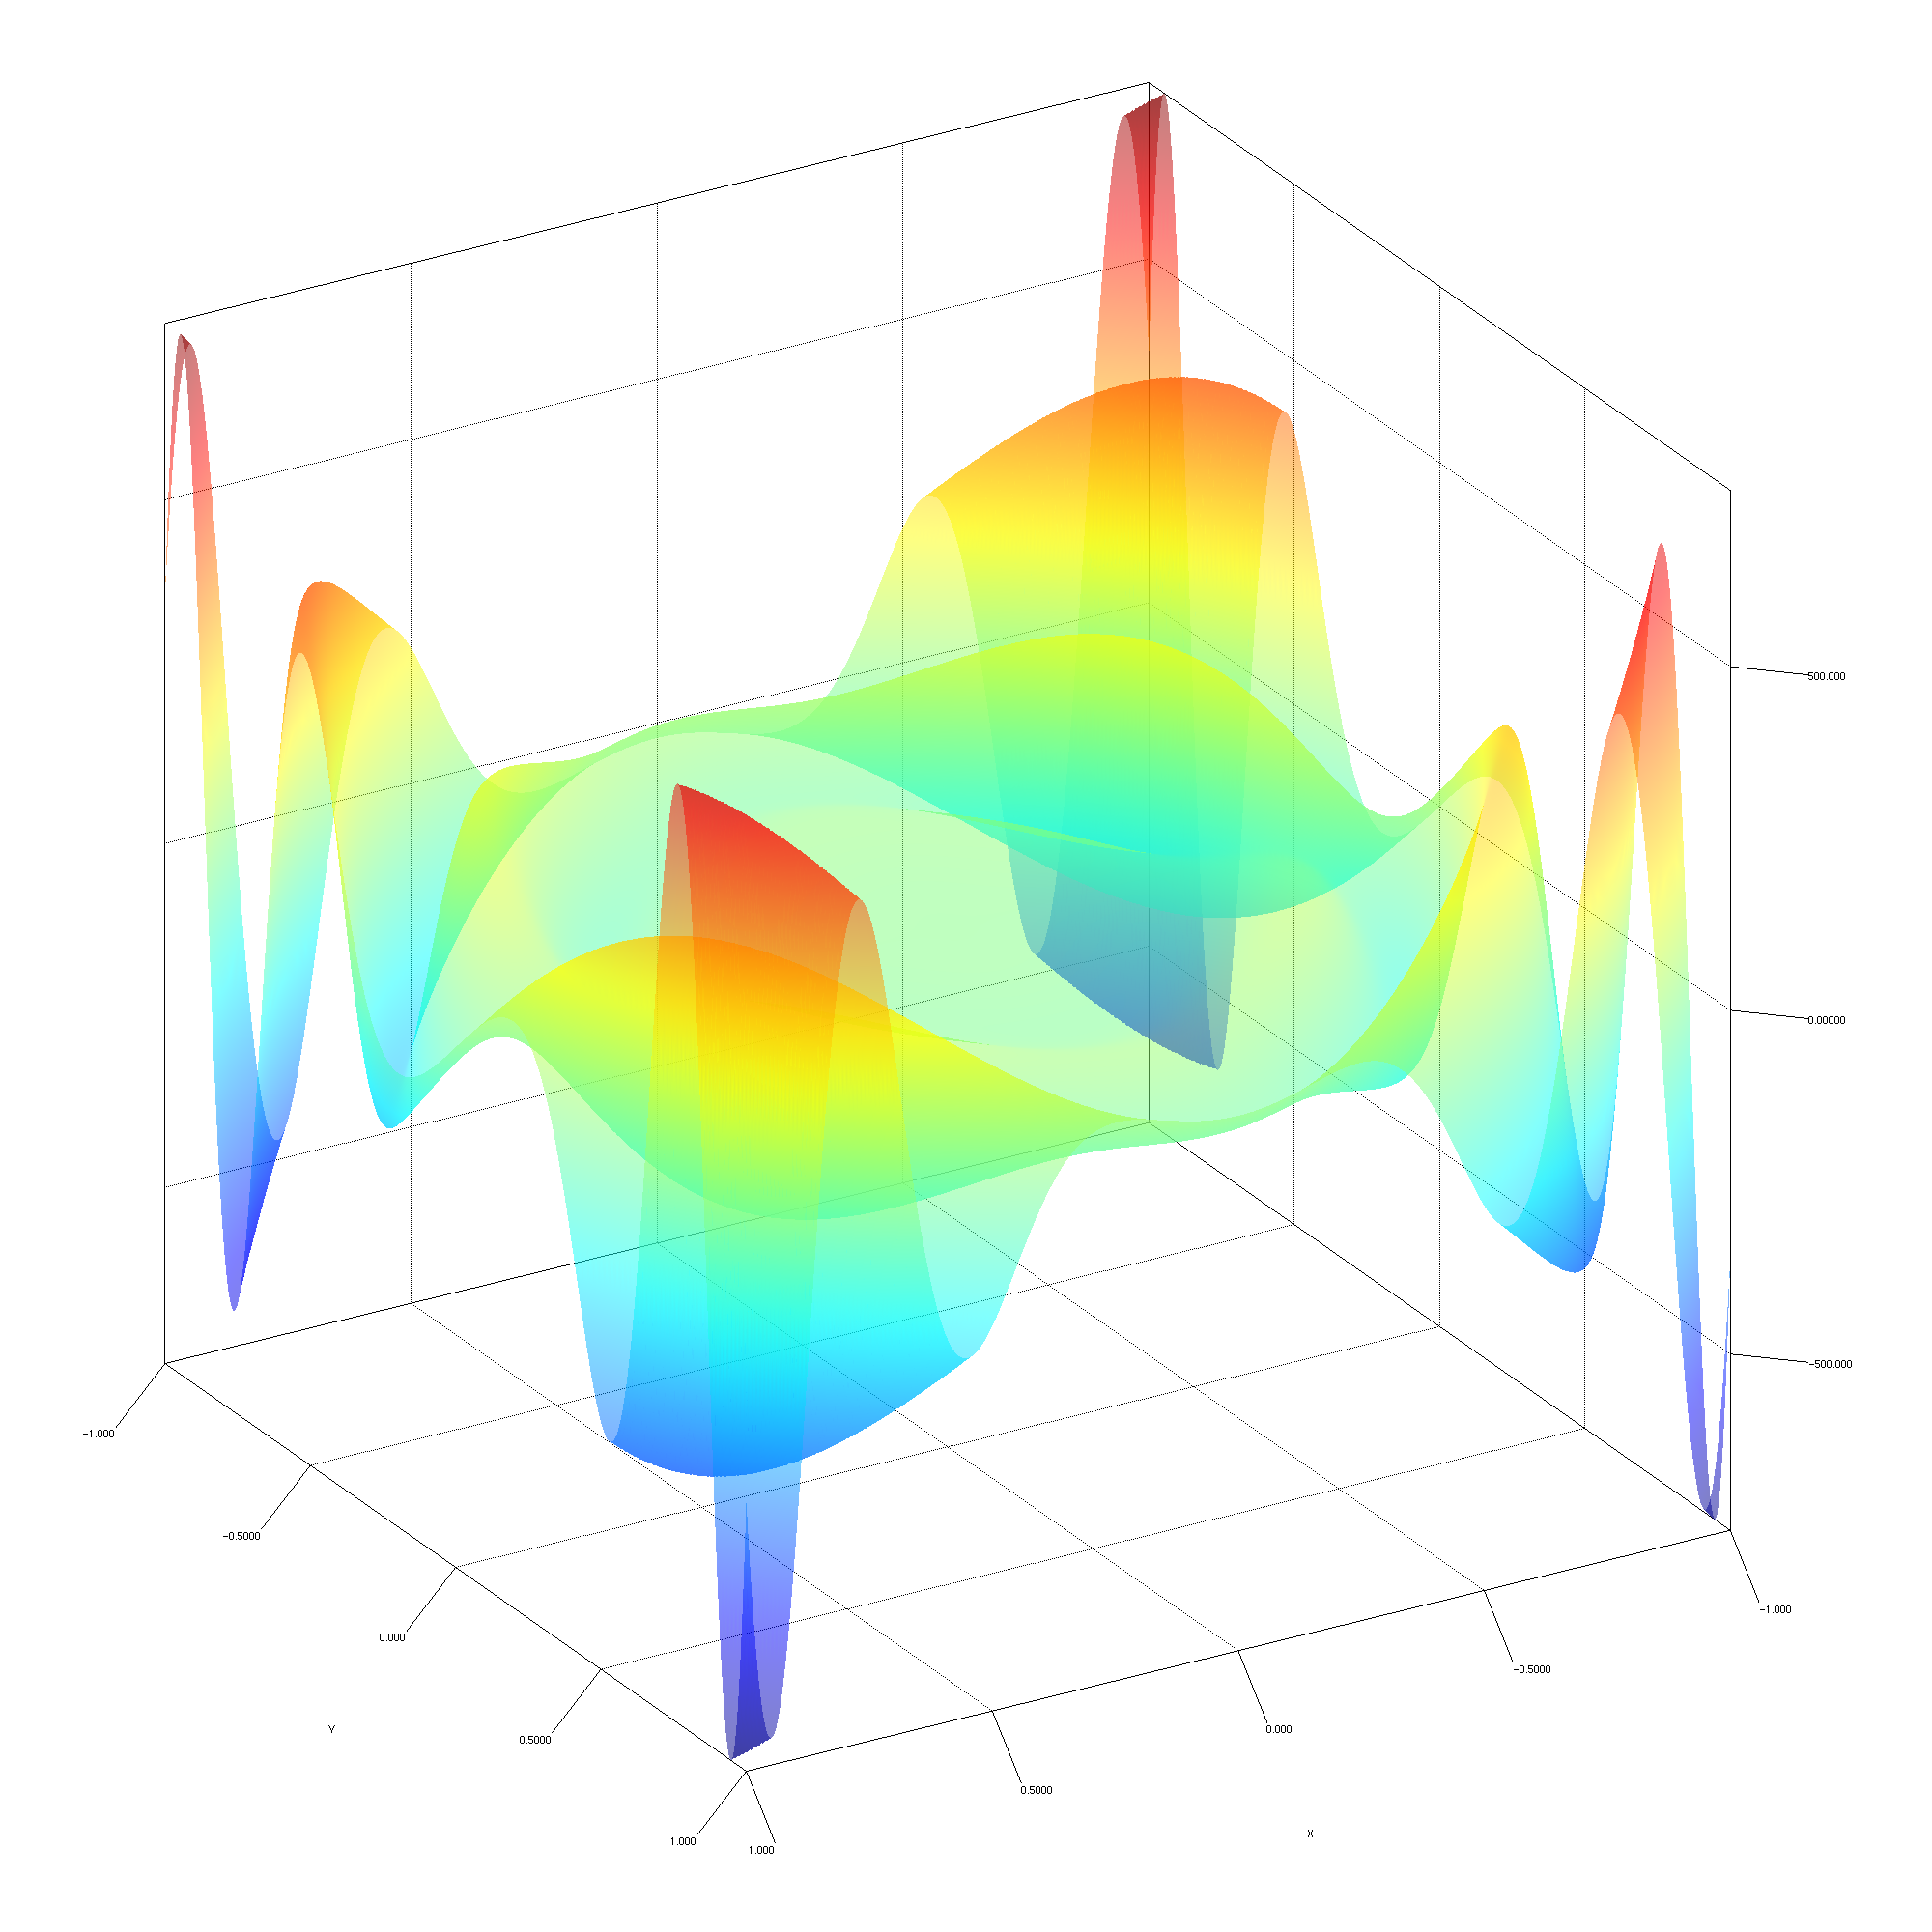
\includegraphics[scale=0.43]{plot_result.png}
    \caption{Output generated by the program shown in Figure \ref{label:fig1}.}
\end{figure}

Kotlin$\nabla$ treats mathematical functions and programming functions with the same underlying abstraction. Expressions are composed recursively to form a data-flow graph (DFG). An expression is simply a \texttt{Function}, which is only evaluated once invoked with numerical values, e.g. \texttt{z(0, 0)}.

\begin{figure}[!htb]
    \begin{minted}[fontsize=\footnotesize]{kotlin}
        val z = sin(10 * (x * x + pow(y, 2))) / 10
    \end{minted}
    \centering
    \begin{tikzpicture}[grow=left]
        \tikzset{level distance=45pt,sibling distance=-3pt}
        \Tree [.$\div$ [.\texttt{sin} [.$\times$ \texttt{10} [.$+$ [.$\times$ \texttt{\textbf{x}} \texttt{\textbf{x}} ] [.\texttt{pow} \texttt{\textbf{y}} \texttt{2} ] ] ] ] \texttt{10} ]
    \end{tikzpicture}
    \caption{Implicit DFG constructed by the original expression, \texttt{z}.}
\end{figure}

Kotlin$\nabla$ supports shape-shafe tensor operations by encoding tensor rank as a parameter of the operand's type signature. By enumerating type-level integer literals, we can define tensor operations just once using the highest literal, and rely on Liskov substitution to preserve shape safety for subtypes.

\begin{figure}[!htb]
    \begin{minted}[fontsize=\scriptsize]{kotlin}
        // Literals have reified values for runtime comparison
        open class `0`(override val value: Int = 0): `1`(0)
        open class `1`(override val value: Int = 1): `2`(1)
        class `2`(open val value: Int = 2) // Greatest literal
        // <L: `2`> will accept L <= 2 via Liskov substitution
        class Vec<E, L: `2`>(len: L, cts: List<E> = listOf())
        // Define addition for two vectors of type Vec<Int, L>
        operator fun <L: `2`, V: Vec<Int, L>> V.plus(v: V) =
        Vec<Int, L>(len, cts.zip(v.cts).map { it.l + it.r })
        // Type-checked vector addition with shape inference
        val Y = Vec(`2`, listOf(1, 2)) + Vec(`2`, listOf(3, 4))
        val X = Vec(`1`, listOf(1, 2)) + Vec(`3`) // Undefined!
    \end{minted}
    \caption{Shape safe tensor addition for rank-1 tensors, $\forall L\leq2.$}
\end{figure}

It is possible to enforce shape-safe vector construction as well as checked vector arithmetic up to a fixed \texttt{L}, but the full implementation is omitted for brevity. A similar pattern can be applied to matrices and higher rank tensors, where the type signature encodes the shape of the operand at runtime.

With these basic ingredients, we have almost all the features necessary to build an expressive shape-safe AD, but unlike prior implementations using Scala or Haskell, in a language that is fully interoperable with Java, while also capable of compiling to JVM bytecode, JavaScript, and native code.

In future work, we intend to implement a full grammar of differentiable primitives including matrix convolution, control flow and recursion. While Kotlin$\nabla$ currently implements arithmetic manually, we plan to wrap a BLAS such as cuBLAS or native linear algebra library for performance.

\section{Type system}

Describing the Kotlin$\nabla$ type system (formally).

{\tiny
\begin{table}[H]
    \begin{tabular}{|c|c|c|c|l|}
        \hline
        \multicolumn{1}{|c|}{Math}                            &  Infix                                                                         &  Prefix                                                                                 & Postfix                                                                                    & Type                                                                                                                                                                                     \\ \hline
                 $A + B$                                      & \begin{tabular}{@{}c@{}}\texttt{a + b}\\\texttt{a.plus(b)}\end{tabular}        &  \texttt{plus(a, b)}                                                                    &                                                                                            & $ (\texttt{a}:  \mathbb{R}^{\tau}\rightarrow\mathbb{R}^{\pi}, \texttt{b}: \mathbb{R}^{\lambda} \rightarrow \mathbb{R}^{\pi}) \rightarrow (\mathbb{R}^{?}\rightarrow \mathbb{R}^{\pi}) $ \\ \hline
                 $A - B$                                      & \begin{tabular}{@{}c@{}}\texttt{a - b}\\\texttt{a.minus(b)}\end{tabular}       &  \texttt{minus(a, b)}                                                                   &                                                                                            & $ (\texttt{a}:  \mathbb{R}^{\tau}\rightarrow\mathbb{R}^{\pi}, \texttt{b}: \mathbb{R}^{\lambda} \rightarrow \mathbb{R}^{\pi}) \rightarrow (\mathbb{R}^{?}\rightarrow\mathbb{R}^{\pi})  $ \\ \hline
                 $A   B$                                      & \begin{tabular}{@{}c@{}}\texttt{a * b}\\\texttt{a.times(b)}\end{tabular}       &  \texttt{times(a, b)}                                                                   &                                                                                            & $ (\texttt{a}: \mathbb{R}^{\tau}\rightarrow\mathbb{R}^{m*n}, \texttt{b}: \mathbb{R}^{\lambda}\rightarrow\mathbb{R}^{n*p})    \rightarrow (\mathbb{R}^{?}\rightarrow\mathbb{R}^{m*p})  $ \\ \hline
\begin{tabular}{@{}c@{}}$\frac{A}{B}$\\$AB^{-1}$\end{tabular} & \begin{tabular}{@{}c@{}}\texttt{a / b}\\\texttt{a.div(b)}\end{tabular}         &  \texttt{div(a, b)}                                                                     &                                                                                            & $ (\texttt{a}: \mathbb{R}^{\tau}\rightarrow\mathbb{R}^{m*n}, \texttt{b}: \mathbb{R}^{\lambda}\rightarrow\mathbb{R}^{p*n}) \rightarrow (\mathbb{R}^{?}\rightarrow\mathbb{R}^{m*p})     $ \\ \hline
\begin{tabular}{@{}c@{}}$-A$\\$+A$\end{tabular}               &                                                                                &  \begin{tabular}{@{}c@{}}\texttt{-a}\\\texttt{+a}\end{tabular}                          & \begin{tabular}{@{}c@{}}\texttt{a.unaryMinus()}\\\texttt{a.unaryPlus()}\end{tabular}       & $                   (\texttt{a}: \mathbb{R}^{\tau}\rightarrow\mathbb{R}^{\pi}) \rightarrow (\mathbb{R}^{\tau}\rightarrow\mathbb{R}^{\pi})                                             $ \\ \hline
\begin{tabular}{@{}c@{}}A+1 \\ A-1\end{tabular}               & \begin{tabular}{@{}c@{}}\texttt{a + 1}\\\texttt{a - 1}\end{tabular}            &  \begin{tabular}{@{}c@{}}\texttt{++a}\\\texttt{--a}\end{tabular}                        & \begin{tabular}{@{}c@{}}\texttt{a++, a.inc()}\\\texttt{a--, a.dec()}\end{tabular}          & $                 (\texttt{a}: \mathbb{R}^{\tau}\rightarrow\mathbb{R}^{m*m}) \rightarrow (\mathbb{R}^{\tau}\rightarrow\mathbb{R}^{m*m})                                               $ \\ \hline
\begin{tabular}{@{}c@{}}sin(a)\\cos(a)\\tan(a)\end{tabular}   &                                                                                &  \begin{tabular}{@{}c@{}}\texttt{sin(a)}\\\texttt{cos(a)}\\\texttt{tan(a)}\end{tabular} & \begin{tabular}{@{}c@{}}\texttt{a.sin()}\\\texttt{a.cos()}\\\texttt{a.tan()}\end{tabular}  & $                                            (\texttt{a}: \mathbb{R}\rightarrow\mathbb{R}) \rightarrow (\mathbb{R}\rightarrow\mathbb{R})                                              $ \\ \hline
                $\ln(A)$                                      &                                                                                &  \begin{tabular}{@{}c@{}}\texttt{ln(a)}\\\texttt{log(a)}\end{tabular}                   & \begin{tabular}{@{}c@{}}\texttt{a.ln()}\\\texttt{a.log()}\end{tabular}                     & $                  (\texttt{a}: \mathbb{R}^{\tau}\rightarrow\mathbb{R}^{m*m}) \rightarrow (\mathbb{R}^{\tau}\rightarrow\mathbb{R}^{m*m})                                              $ \\ \hline
               $\log_b A$                                     & \texttt{a.log(b)}                                                              &  \texttt{log(a, b)}                                                                     &                                                                                            & $       (\texttt{a}: \mathbb{R}^{\tau}\rightarrow\mathbb{R}^{m*m}, \texttt{b}: \mathbb{R}^{\lambda}\rightarrow\mathbb{R}^{m*m}) \rightarrow (\mathbb{R}^{?}\rightarrow\mathbb{R})     $ \\ \hline
                $A^{b}$                                       & \texttt{a.pow(b)}                                                              &  \tettt{pow(a, b)}                                                                      &                                                                                            & $       (\texttt{a}: \mathbb{R}^{\tau}\rightarrow\mathbb{R}^{m*m}, \texttt{b}: \mathbb{R}^{\lambda}\rightarrow\mathbb{R}) \rightarrow (\mathbb{R}^{?}\rightarrow\mathbb{R}^{m*m})     $ \\ \hline
\begin{tabular}{@{}c@{}}$\sqrt{a}$\\$sqrt[3](a)$\end{tabular} & \begin{tabular}{@{}c@{}}\texttt{a.pow(1.0/2)}\\\texttt{a.root(3)}\end{tabular} &  \begin{tabular}{@{}c@{}}\texttt{a.pow(1.0/2)}\\\texttt{a.root(3)}\end{tabular}         & \begin{tabular}{@{}c@{}}\texttt{a.sqrt()}\\\texttt{a.cbrt()}\end{tabular}                  & $                        (\texttt{a}: \mathbb{R}^{\tau}\rightarrow\mathbb{R}^{m*m}) \rightarrow (\mathbb{R}\rightarrow\mathbb{R}^{m*m})                                               $ \\ \hline
\begin{tabular}{@{}c@{}}$\frac{da}{db}$\\$a'(b)$\end{tabular} & \texttt{a.diff(b)}                                                             &  \texttt{grad(a)[b]}                                                                    & \texttt{d(a) / d(b)}                                                                       & $                    (\texttt{a}: C(\mathbb{R}^{m})^{*}, \texttt{b}: \mathbb{R}\rightarrow\mathbb{R}) \rightarrow (\mathbb{R}^{m}\rightarrow\mathbb{R})                               $ \\ \hline
               $\nabla a$                                     &                                                                                &  \texttt{grad(a)}                                                                       & \texttt{a.grad()}                                                                          & $                   (\texttt{a}: C(\mathbb{R}^{m})^{*}) \rightarrow (\mathbb{R}^{m}\rightarrow\mathbb{R}^{m})                                                                         $ \\ \hline
    \end{tabular}
\end{table}
}

\section{Differentiable programming}

The renaissance of modern deep learning is widely credited to progress in three research areas: algorithms, data and hardware. Among algorithms, most research has focused on deep learning architectures and representation learning. Equally important, arguably, is the role that automatic differentiation (AD) has played in facilitating the implementation of these ideas. Prior to the adoption of general-purpose AD libraries like Theano, PyTorch and TensorFlow, gradients needed to be programmed manually. The emergence of these and other libraries specifically tailored to deep learning simplified and accelerated the pace of machine learning, allowing researchers to focus on gradient-based optimization, network architectures and learning representations. Some of these ideas in turn, formed the basis for new methods in automatic differentiation, which continues to be an active area of research.

In deep learning, research primarily focuses on differentiable representations. In contrast, many problems we would like to solve are non-differentiable in their natural domain. For example, the structure of character-based representations are not easily differentiable as small changes to a word's symbolic representation can cause large differences to its semantic meaning. A key insight from deep learning research is that many problems require posing a good representation. For example, if we can represent words as a vector of real numbers, so that relations between words are spatially preserved by the vector representation, then we can perform gradient descent on such a space. Many classes of discrete problems can be relaxed to continuous surrogates by introducing a good representation.

As more domains found efficient representations, researchers observed neural networks were part of a broader class of differentiable architectures that could be built and interpreted in a manner not unlike computer programming [1], [2]. Hence the term \textit{differentiable programming} was born.

\chapter{Verification and validation}

How do we test a machine that learns?

\section{Adversarial test case generation}

Neural networks and differentiable programming has provided a powerful new set of optimization tools for training learning algorithms. However these methods are often brittle to small variations in the input space, and have difficulty with generalization. In contrast, these same techniques used for probing the failure modes of neural networks can be applied to adversarial test case generation for traditional programs.

\section{Background}

Suppose we have a program $P: \mathbb{R}\rightarrow\mathbb{R}$ where:
%
\begin{equation}
    P(x)=p_n \circ p_{n-1} \circ p_{n-2} \circ ... \circ p_1 \circ p_0
\end{equation}
%
From the chain rule of calculus, we know that:
%
\begin{equation}
    \frac{dP}{dp_0} = {\displaystyle \prod_{i=1}^{n} \frac{dp_{i}}{dp_{i-1}}}
\end{equation}

%
% Imagine a set of tests $\mathrm{T}: \mathbb{R} \rightarrow \mathbb{B}$ where $\mathrm{T}={\tau_1, ...\tau_m}$.  For example,
%
Imagine a single test $T: \mathbb{R} \rightarrow \mathbb{B}$. Consider the following example::
%
\begin{equation}
    T: \forall x \in (0, 1), P(x) < C
\end{equation}
%
How can we find a set of inputs that break the test under a fixed computational budget (i.e. constant number of program evaluations)? In other words:
%
\begin{equation}
    D_T: \{ x^i \sim \mathbb{R}(0, 1) \mid P(x^i) \implies \neg T \}, maximize |D_T|
\end{equation}
%
If we have no information about the program implementation or its input distribution, $D_P$, we can do no better than random search (cf. no free lunch). However, if we know something about the input distribution, we could re-parameterize the distribution to incorporate our knowledge. Assuming the program already works on most common inputs (e.g. from a training set), we might want to sample $x \sim \frac{1}{D_P}$ for inputs that are infrequent, although this strategy is not guaranteed to yield any additional failures. If we knew how $P$ were implemented, we might be able prioritize our search in input regions leading towards internal discontinuities (e.g. edge cases in software testing). However for functions that are continuous and differentiable, these heuristics are almost certainly insufficient. Finally, we could train a neural network to predict inputs that were likely to cause a program to fail a given specification. As input, the network would take the function and test cases, and as its output, produce values that were likely to violate $T$.

Another strategy, independent of how candidate inputs are selected, is to use some form of gradient based optimization in the search procedure. For example in (3) we could have a loss function:
%
\begin{equation}
    \mathcal{L}(P, x) = C - P(x)
\end{equation}
%
The gradient of the loss w.r.t. $x$ (assuming $P$ is fixed\footnote{In contrast with backpropogation, where the parameters are updated.}) is:
%
\begin{equation}
    \nabla \mathcal{L}(P, x) = - \frac{dP}{dx}
\end{equation}
%
Where the vanilla gradient update step is defined as:
%
\begin{equation}
    x_{n+1}^i=x_{n}^i - \alpha\frac{dP}{dx}
\end{equation}
%
We hypothesize that if the implementation of $P$ were flawed and a counterexample to (3) existed, as sample size increased, a subset of gradient descent trajectories would fail to converge, a portion would converge to local minima, and a subset of trajectories would discover inputs violating the program specification. How would such a search procedure look in practice? Consider the following:

% Furthermore, we hypothesize that if a sufficiently large fraction of the input space existed where $T$ were false, then as we sample from that space, the probability of detection would approach 1:
%
% \begin{equation}
%     (\forall i \in I^\dagger, p(i) \implies \neg T) \implies \lim_{|x|\to \infty}Prob(\hat{T}=False) = 1
% \end{equation}
%


\begin{algorithm}
    \SetKwInOut{Input}{Input}
    \SetKwInOut{Output}{Output}

    \Input{Program $P$, specification $T$, evaluation budget $Budget$}
    \Output{$D_T$, the set of inputs which cause $P$ to fail on T}
    $D_T$ = []\;
    evalCount = 0\;
    \While{evalCount \leq $Budget$} {
    sample candidate input $x^i$ according to selection strategy S\;
    \eIf{$P(x^i)\implies$ \neg T}{
    append $x^i$ to D_T\;

    }{
    n = 0\;
    $x^i_n = x^i$\;

    \While{$n \leq C \land evalCount \leq Budget$ \land $\neg converged$} {
    n++\;

    $x_{n}^i=x_{n-1}^i - \alpha\frac{dP}{dx}$\;


    \If{P(x^i_n) \implies T} {
    append $x^i_n$ to D_T\;

    break\;

    }

    evalCount++\;
    }
    }
    evalCount++; i++\;
    }

    \caption{Algorithm for finding test failures. First select a candidate input $x^i$ according to sampling strategy $S$ (e.g. uniform random, or a neural network which takes $P$ and $T$ as input). If $P(x^i)$ violates $T$, we can append $x^i$ to $D_T$ and repeat. Otherwise, we follow the gradient of $\mathcal{L}(P, x)$ with respect to $x$ and repeat until test failure, gradient descent convergence, or a fixed number of G.D. steps $C$ are reached before resampling $x^{i+1}$ from the initial sampling strategy $S$ to ensure each G.D. trajectory will terminate before exhausting our budget.}
\end{algorithm}

\section{Regression testing: a tool to prevent catastrophic forgetting}

An endemic problem in modern deep learning is the problem of forgetting. In order to combat this issue, we turn to a classic software testing tool: regression testing.

Regular regression testing gives clear diagnostics about the behavior of these systems.

\chapter{Case study: application for autonomous robotics}

Here, we implement a mobile application using the above toolchain.

\section{Design}

Designed with Hatchery.

\section{Implementation}

Implementation includes Kotlin$\nabla$

\section{Verification}

Verified using property-based testing.

\section{Maintenance}

Deployed and CI-tested using Docker.

\chapter{Software reproducibility}

\section{Operating systems and virtualization}

Operating systems are a source of variability. Filesystems are complicated.

\section{Dependency management}

Packages are a source of variability. Dependency hell is NP Complete: https://research.swtch.com/version-sat

\section{Containerization}

One of the challenges of distributed software development across heterogeneous platforms is the problem of variability. With the increasing pace of software development comes the added burden of software maintenance. As hardware and software stacks evolve, so too must source code be updated to build and run correctly. Maintaining a stable and well documented codebase can be a considerable challenge, especially in a robotics setting where contributors are frequently joining and leaving the project. Together, these challenges present significant obstacles to experimental reproducibility and scientific collaboration.

In order to address the issue of software reproducibility, we developed a set of tools and development workflows that draw on best practices in software engineering. These tools are primarily built around containerization, a widely adopted virtualization technology in the software industry. In order to lower the barrier of entry for participants and minimize variability across platforms (e.g. simulators, robotariums, Duckiebots), we provide a state-of-the-art container infrastructure based on Docker, a popular container engine. Docker allows us to construct versioned deployment artifacts that represent the entire filesystem and to manage resource constraints via a sandboxed runtime environment.

\begin{figure}[ht]
    \centering
    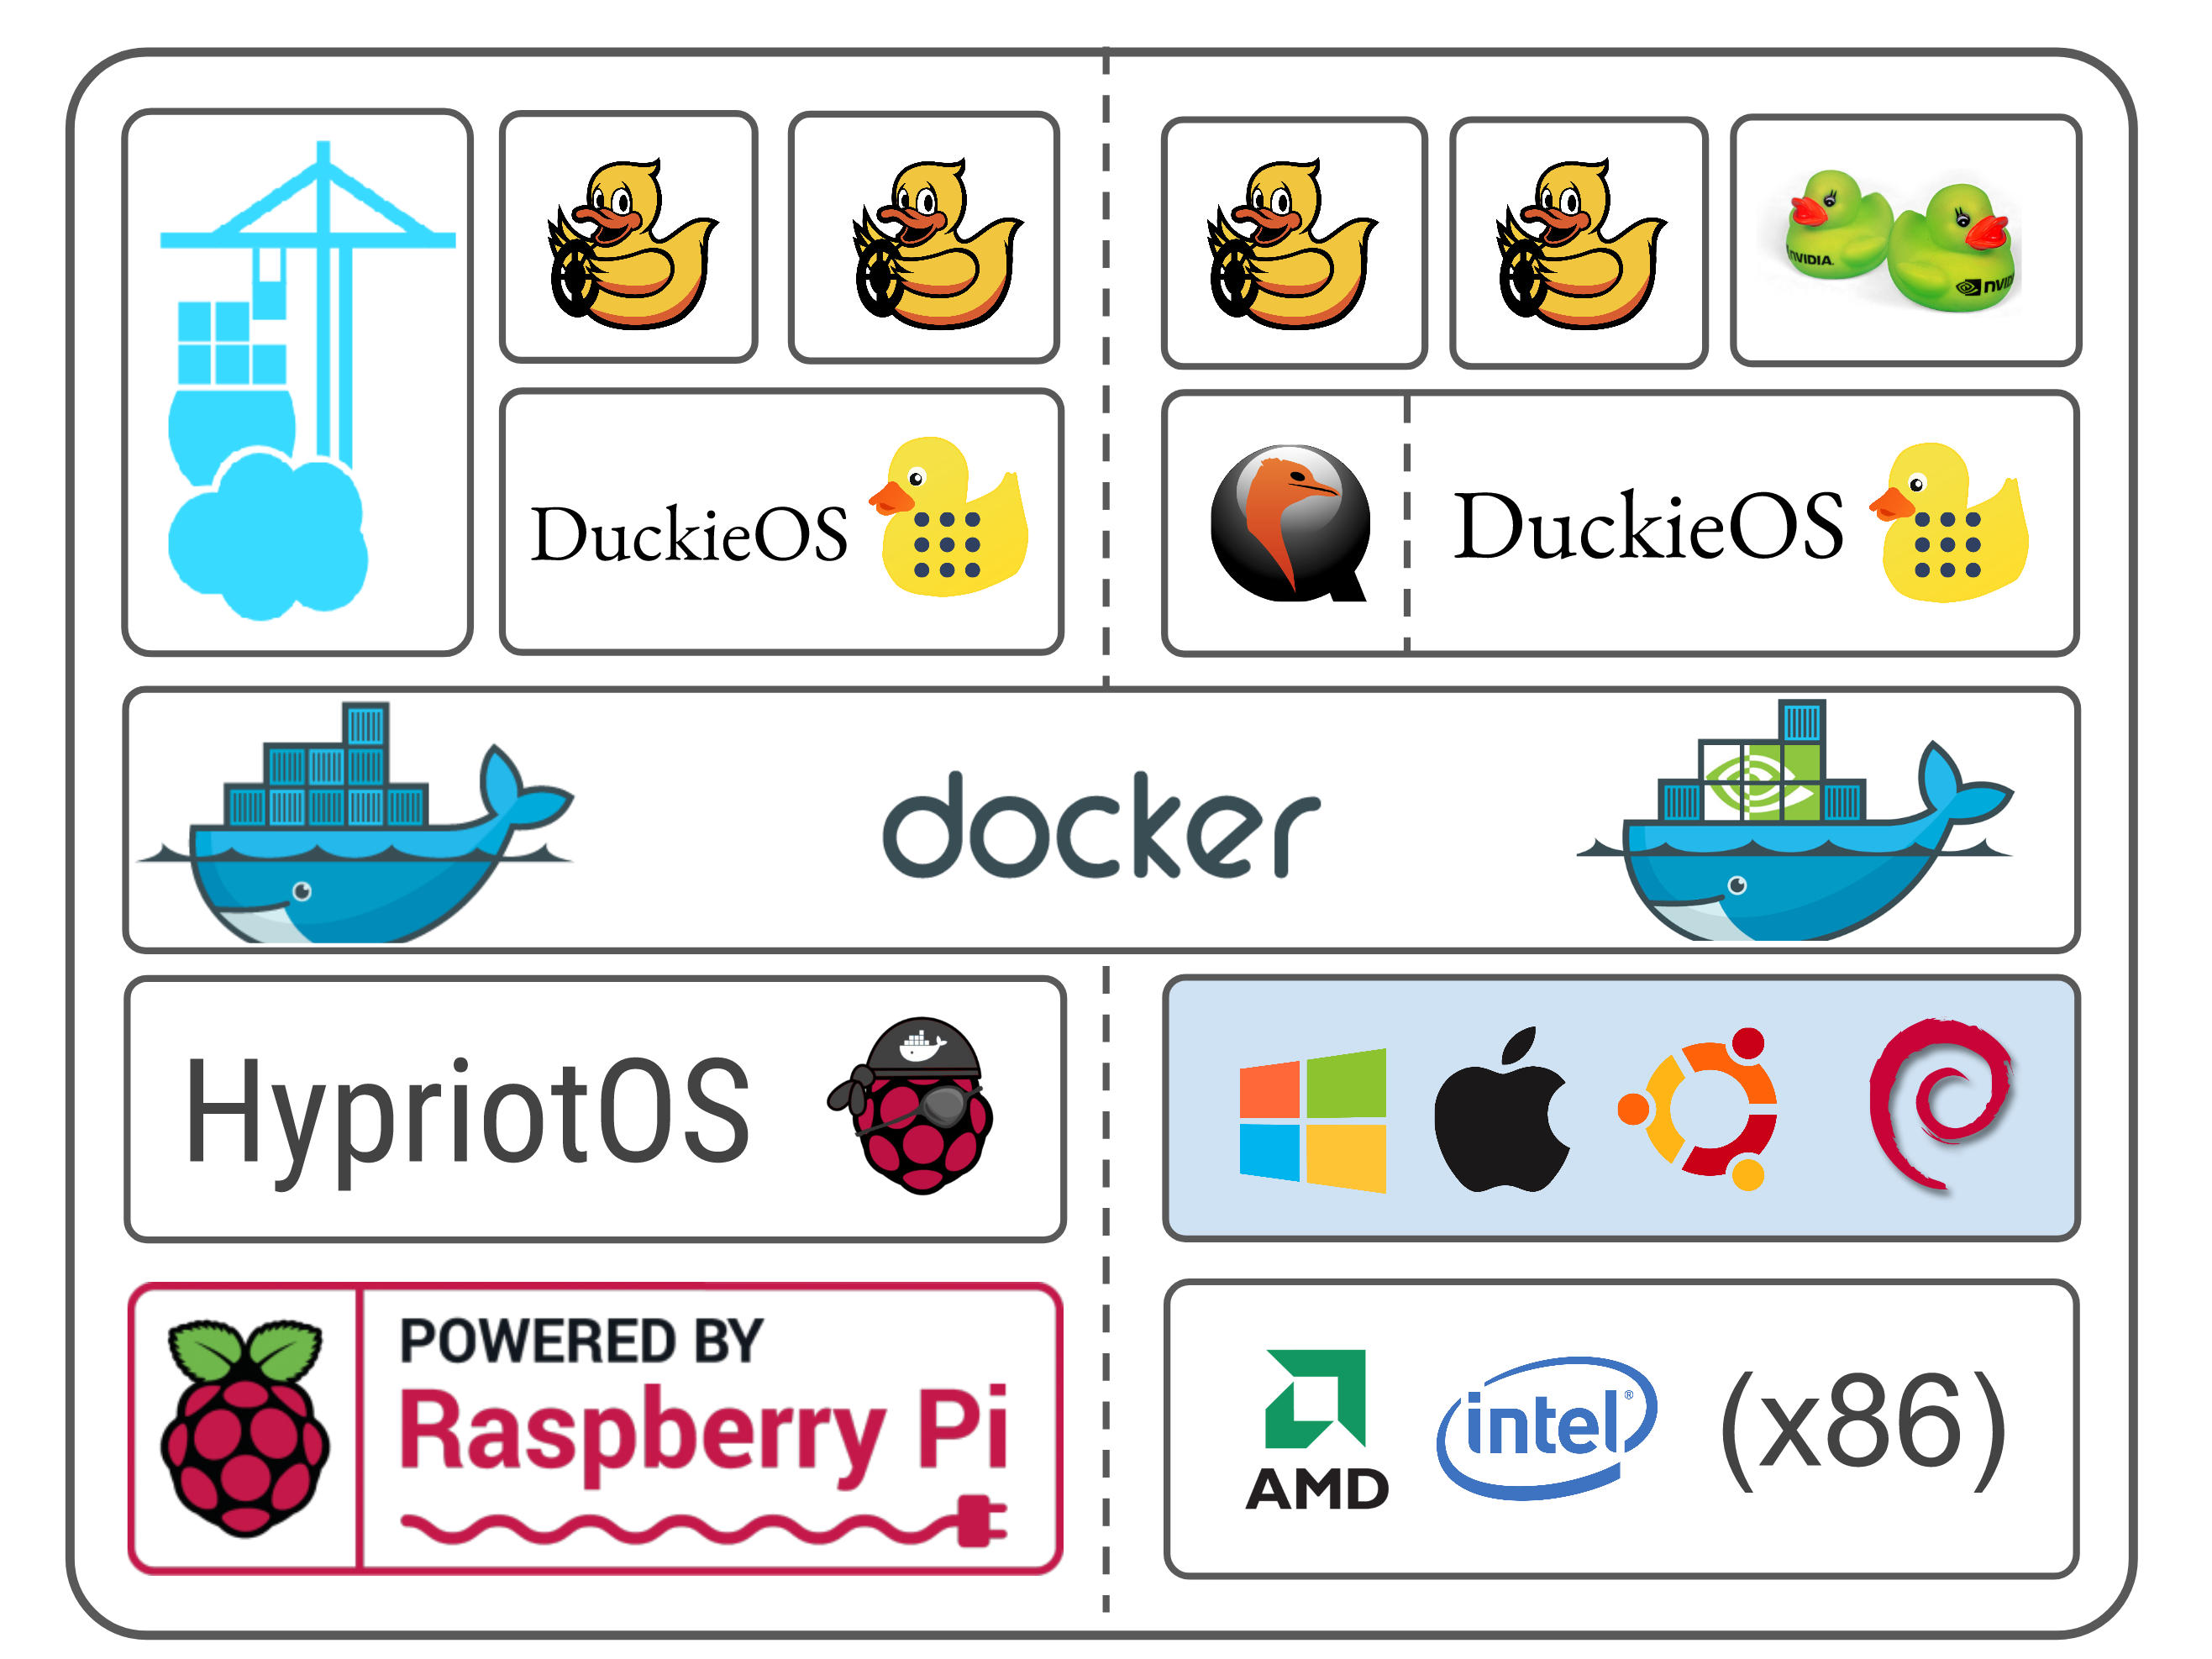
\includegraphics[width=0.45\textwidth]{docker_stack_1.png}
    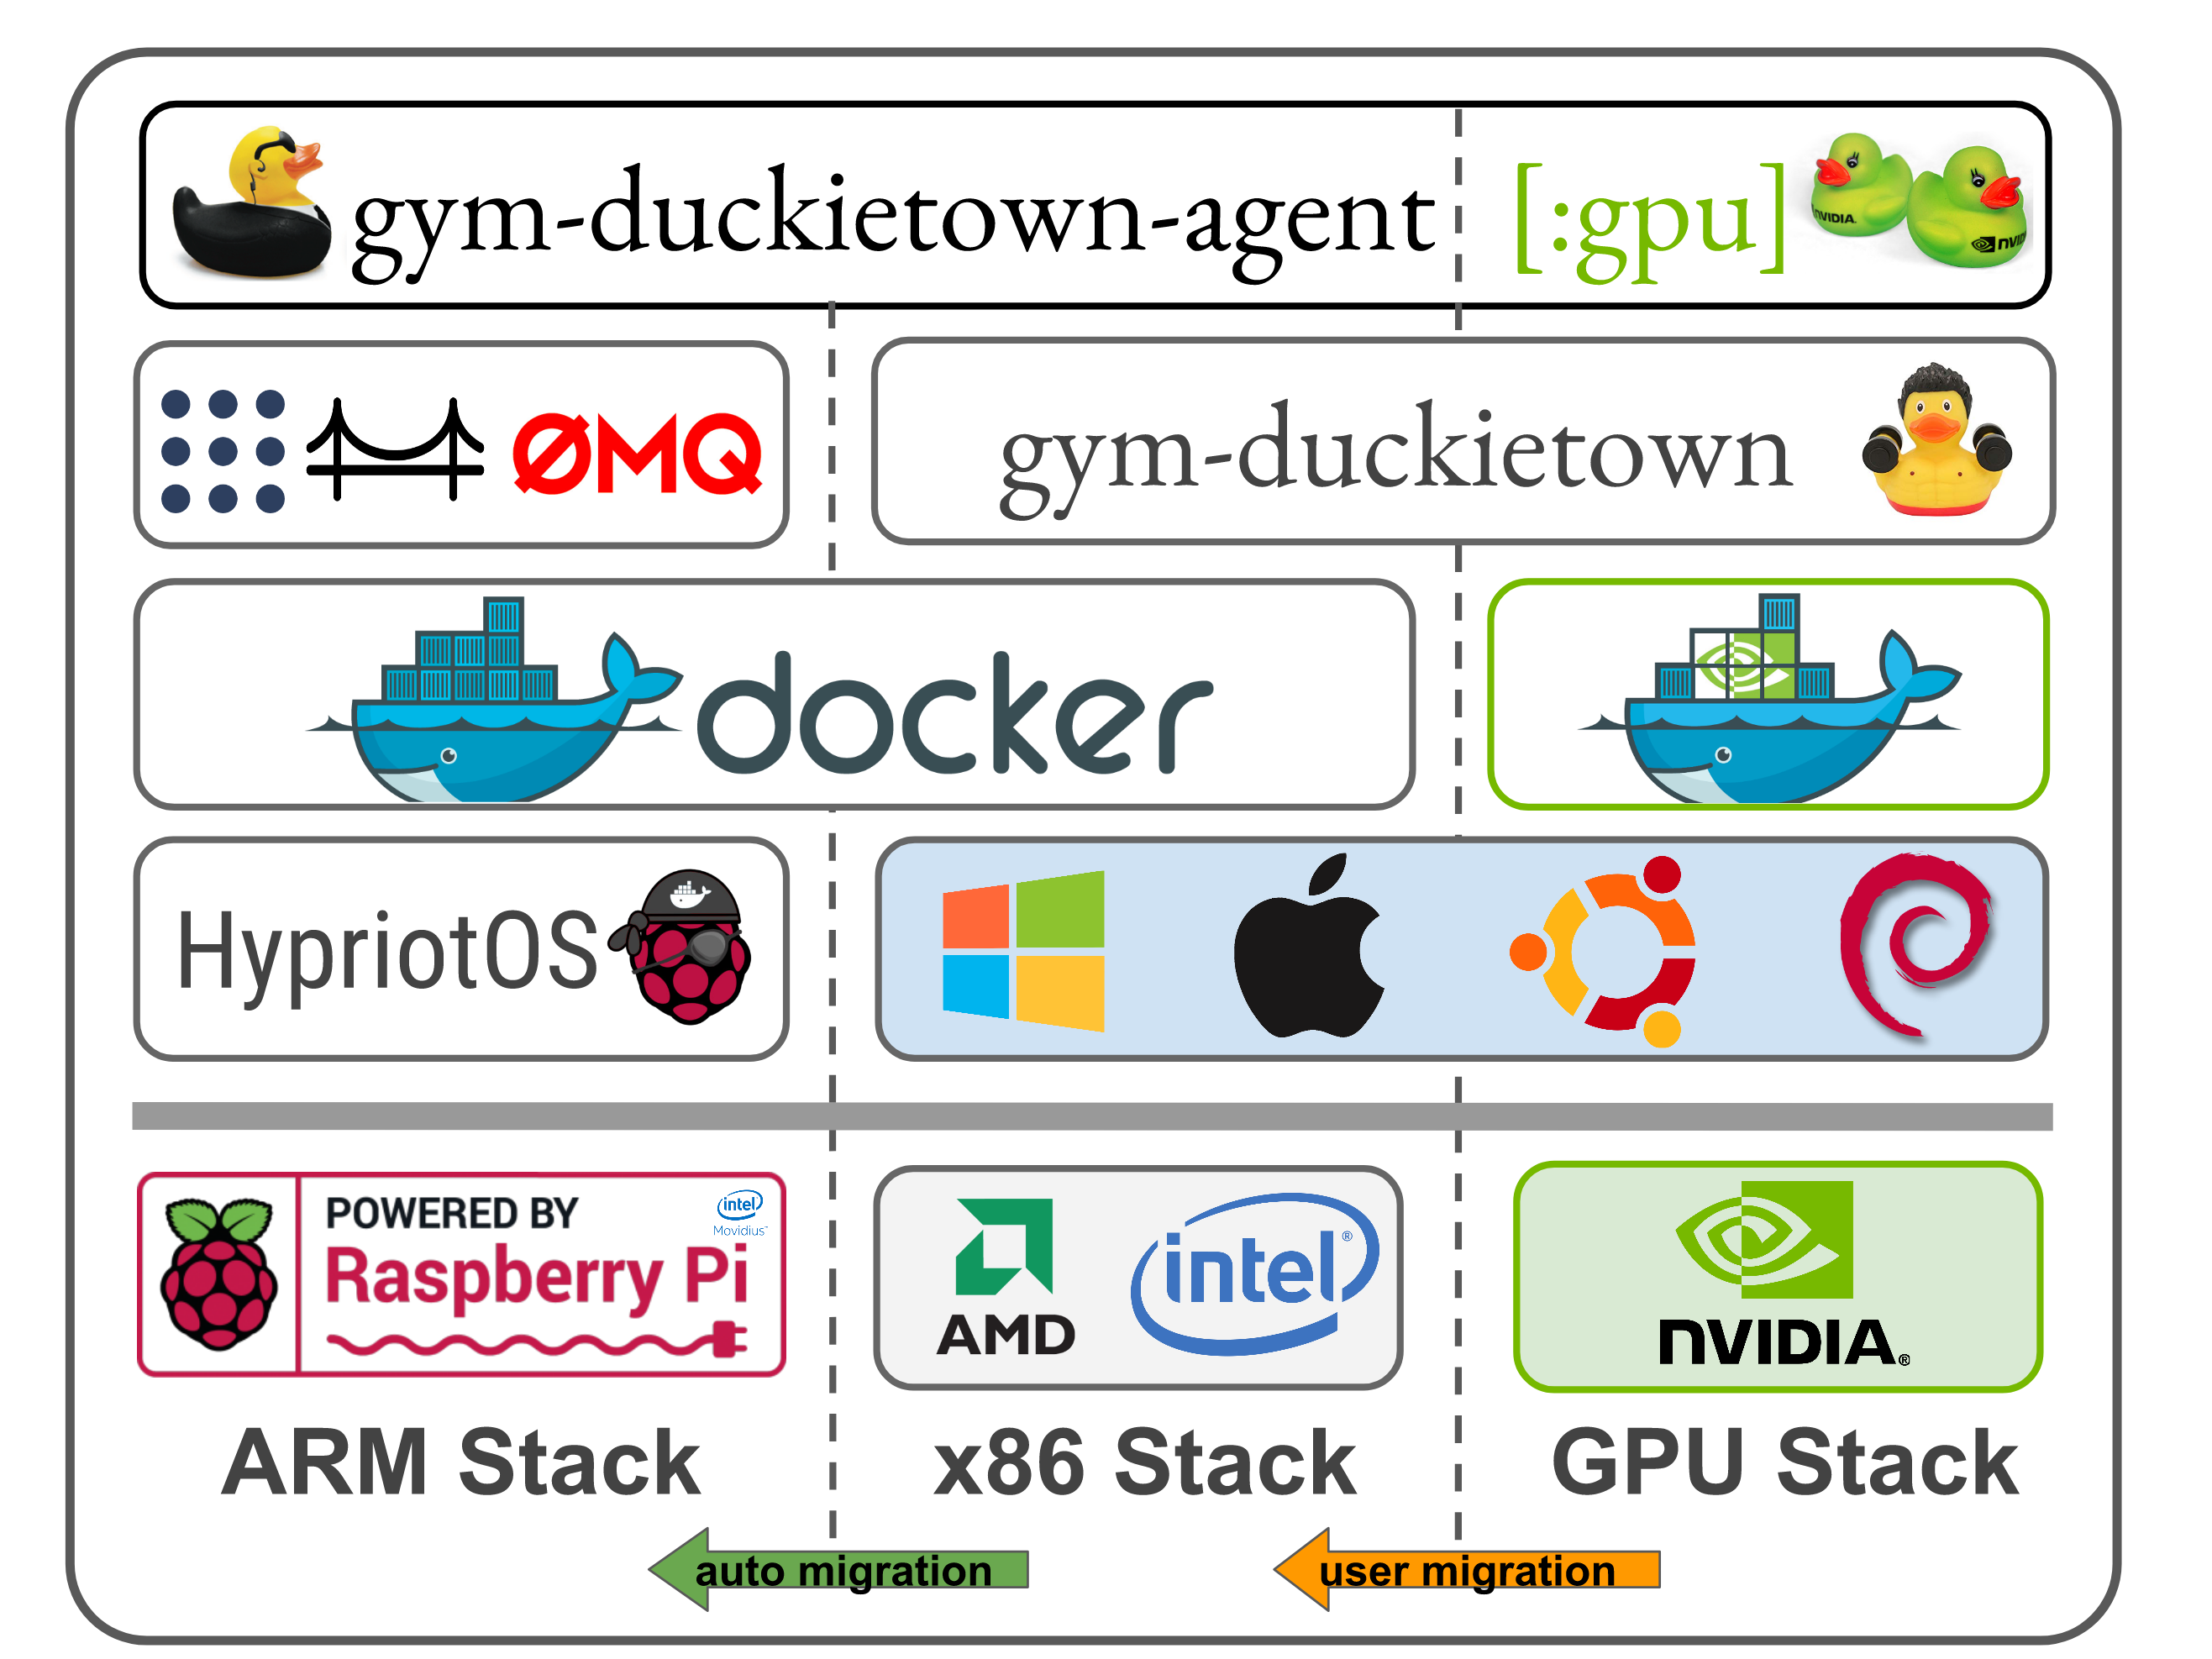
\includegraphics[width=0.45\textwidth]{docker_stack_2.png}
    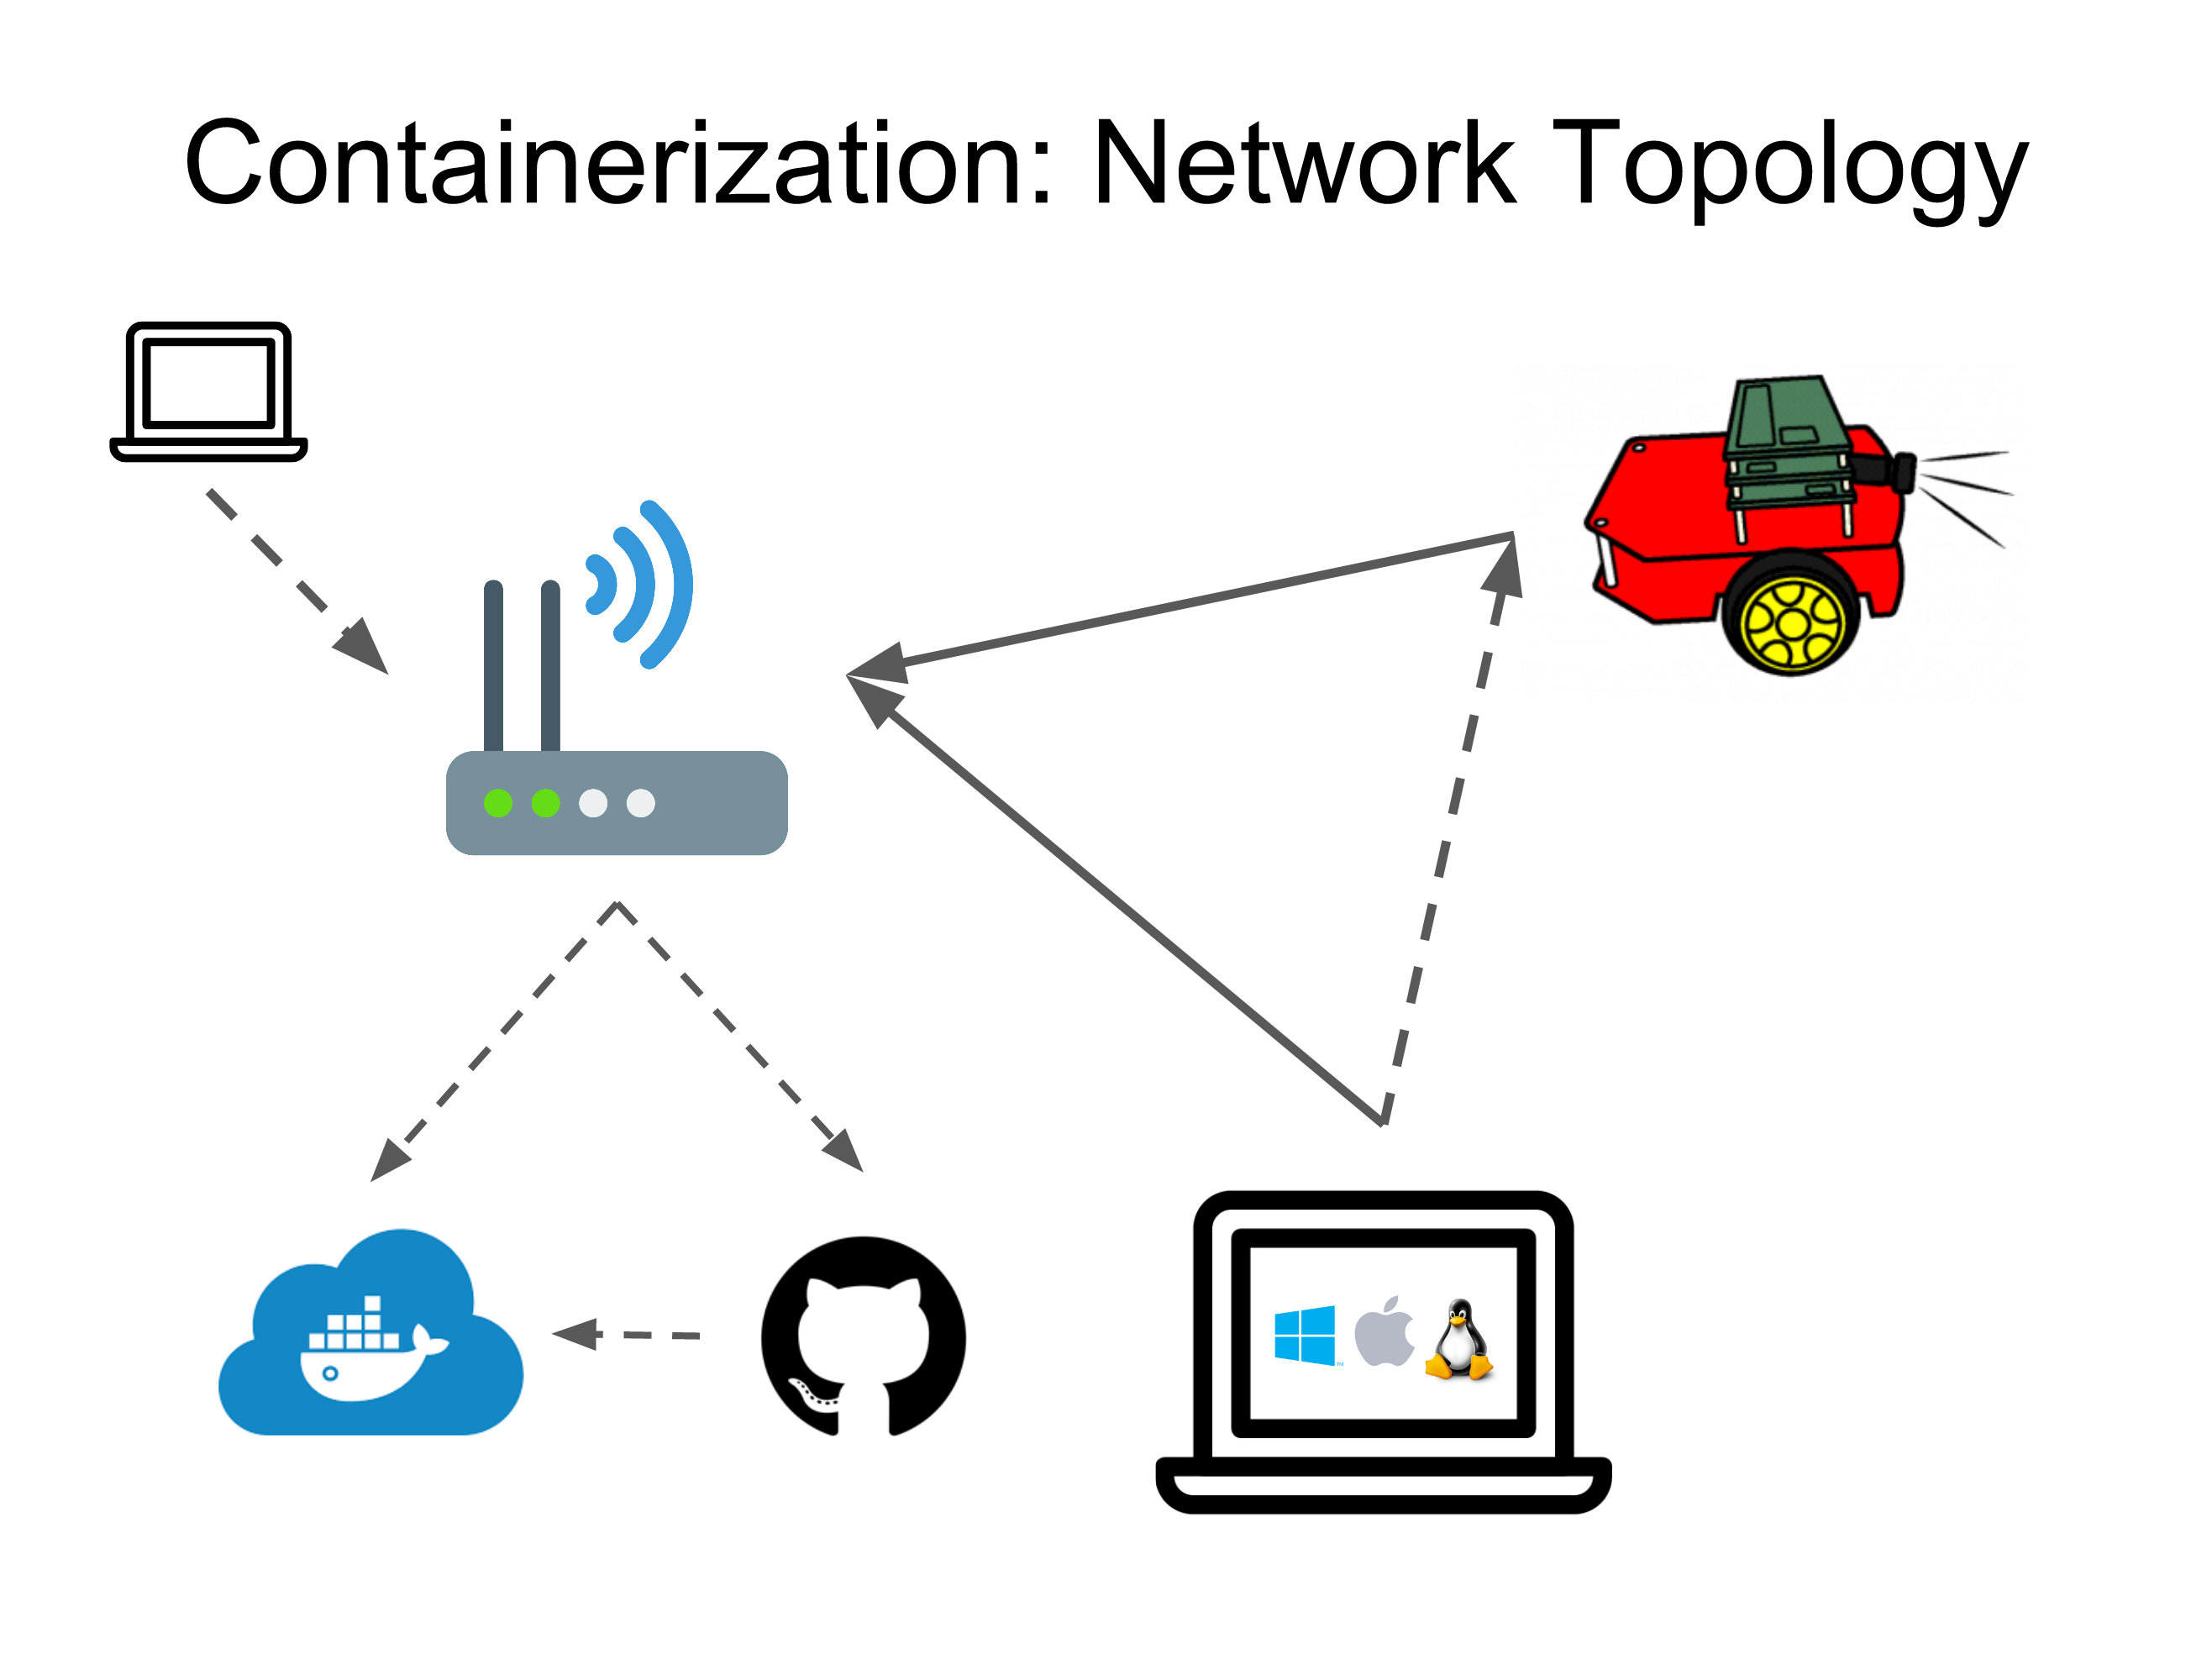
\includegraphics[width=0.35\textwidth]{network_infra.png}
    \caption{AI-DO container infrastructure. Left: The ROS stack targets two primary architectures, x86 and ARM. To simplify the build process, we only build ARM artifacts, and emulate ARM on x86. Right: Reinforcement learning stack. Build artifacts are typically trained on a GPU, and transferred to CPU for evaluation. Deep learning models, depending on their specific architecture, may be run on an ARM device using an Intel NCS.}
    \label{fig:docker}
\end{figure}

The Duckietown platform supports two primary instruction set architectures: x86 and ARM. To ensure the runtime compatibility of Duckietown packages, we cross-build using hardware virtualization to ensure build artifacts can be run on all target architectures. Runtime emulation of foreign artifacts is also possible, using a similar technique.\footnote{For more information, this technique is described in further depth at the following URL: \url{https://www.balena.io/blog/building-arm-containers-on-any-x86-machine-even-dockerhub/}.} For performance and simplicity, we only build ARM artifacts and use emulation where necessary (e.g., on x86 devices). On ARM-native, the base operating system is HypriotOS, a lightweight Debian distribution with built-in support for Docker. For both x86 and ARM-native, Docker is the underlying container platform upon which all user applications are run, inside a container.

Docker containers are sandboxed runtime environments that are portable, reproducible and version controlled. Each environment contains all the software dependencies necessary to run the packaged application(s), but remains isolated from the host OS and file system. Docker provides a mechanism to control the resources each container is permitted to access, and a separate Linux namespace for each container, isolating the network, users, and file system mounts. Unlike virtual machines, container-based virtualization like Docker only requires a lightweight kernel, and can support running many simultaneous containers with close to zero overhead. A single Raspberry Pi is capable of supporting hundreds of running containers.

While containerization considerably simplifies the process of building and deploying applications, it also introduces some additional complexity to the software development lifecycle. Docker, like most container platforms, uses a layered filesystem. This enables Docker to take an existing ``image'' and change it by installing new dependencies or modifying its functionality. Images may be based on a number of lower layers, which must periodically be updated. Care must be taken when designing the development pipeline to ensure that such updates do not silently break a subsequent layer as described earlier in Sec.~\ref{sec:dev-pipeline}.

One issue encountered is the matter of whether to package source code directly inside the container, or to store it separately. If source code is stored separately, a developer can use a shared volume on the host OS for build purposes. In this case, while submissions may be reproducible, they are not easily modified or inspected. The second method is to ship code directly inside the container, where any changes to the source code will trigger a subsequent rebuild, effectively tying the sources and the build artifacts together. Including source code alongside build artifacts also has the benefit of reproducibility and diagnostics. If a competitor requires assistance, troubleshooting becomes much easier when source code is directly accessible. However doing so adds some friction during development, which has caused competitors to struggle with environment setup. One solution is to store all sources on the local development environment and rebuild the Docker environment periodically, copying sources into the image.

\chapter{Conclusion}

\section{Future work}

\subsection{Requirements Engineering}

Often it is not possible, or desirable to summarize the performance of a complex system using a single variable. In multi-objective optimization, we have the notion of pareto-efficiency...

Tranditional software engineering has followed a rigorous process model and testing methodology. This model has guided the development of traditional software engineering, intelligent systems will require a reimagining of these ideas to build systems that adapts to its environment during operation. Intelligent systems are designed with objective functions, which are typically one- or low-dimensional metrics for evaluating the performance of the system. Most often, these take the form of a single criteria, such as an \textit{error} or \textit{loss} which can represent descriptive phenomena such as latency, safety, energy efficiency or any number of objective measures.

For example, in the design of a web based advertisement recommendation system, we can optimize for various objectives such as click rate, engagement, sales conversion. So long as we can measure these parameters, with today's powerful function approximators, we can optimize for any singly criterion or combination thereof. Much of the work involved in machine learning is to find representations which are amenable to learning, and preventing unintended consequences. For example, by optimizing for click rate, we create an artificial market for click bots. Similarly, in self driving cars, we often want to optimize for passenger safety. However by doing so naively, we create a vehicle that never moves, or always yields to nearby vehicles.

When building intelligent system developers must first ask, what are the requirements of the system? This process is often the most troublesome part, because the requirements must not be fuzzy specifications like traditional software engineering, but precise, programmable directives. "I would like the system to be fast," is not sufficiently precise. These kinds of requirements must be translated into statistical loss functions, so we must be very precise about how we specify our requirements. If we simply say, "The system must produce a valid response as quickly as possible, in less than 100ms," is better, but leaves open the possibility of returning an empty response.

In traditional software engineering, it is reasonable to assume the people who are implementing the system have some implicit knowledge and are generally well-intentioned human beings working towards the same goal. When building an intelligent system, a more reasonable assumption is that the entity implementing our requirements is a naive but powerful genie, and possibly an adversary. If we are to give it an optimization metric, it will take every conceivable shortcut to achieve that metric. If we are not careful about requirements engineering, this entity can produce a system that does not work, or has unintended consequences.

In the strictest sense, designing a good set of requirements is indistinguishable from implementing the system. With the right language abstractions (e.g. declarative programming), requirements and implementation can be the same thing. These ideas have been explored in recent decades with languages like SQL and Prolog. While these are toy systems, neural networks can express much larger classes of functions than traditional software engineering.

\subsection{Continuous Delivery and Continual Learning}

In CI/CD, software artifacts are "continously" updated. Similarly, intelligent systems must continously adapt to their environment and this trend will only accelerate.

Incremenental updates will grow increasingly smaller, until the program starts to alter itself after every input it processes.

We need tools to more effectively harness the stochasticity of these learning systems.

\subsection{Developers, Operations, and the DevOps toolchain}

Software engineers have begun to realize the value of bespoke tools that facilitate the process of shipping software, in addition to the software itself.

Teams building software are cybernetic systems, and require meta-programs for building code and organizational processes which enable them to ship code more efficiently.

\bibliography{ref}
\bibliographystyle{plain}
\end{document}